% ---------------------------------------------------------
% Project: PhD KAPPA
% File: background.pca.tex
% Author: Andrea Discacciati
%
% Purpose: Section PCa (background)
% ---------------------------------------------------------

\section{Prostate cancer}

% Disease description
%\subsection{Disease description}
Prostate cancer is the development of cancer in the prostate, a gland in the male reproductive system that is located just below the bladder, surrounding the urethra. More than 90\% of all prostate cancers develop from the gland cells and are referred to as adenocarcinomas.

Early prostate cancer is generally asymptomatic. However, symptoms include increased frequency of urination, painful urination (dysuria), blood in the urine (hematuria), and erection dysfunction. This group of symptoms is known as lower urinary tract symptoms. If the cancer has metastasized to the bones, it can also cause bone pain, especially in the vertebrae, ribs, or pelvis.

Prostate cancer is a very heterogeneous disease, ranging from indolent and slow-growing tumors to aggressive and fast-developing tumors (figure \ref{fig:heterogeneitypca}). The majority of prostatic carcinomas are, however, slow-growing and the time period between onset and clinical presentation of the disease can span several years. Men with this subtype of disease are likely to die from unrelated causes, such as cardiovascular diseases. On the other extreme there are aggressive cancers, which grow fast and may metastasize to the bone or lymph nodes, eventually causing premature death. Figure \ref{fig:naturalcourse} schematically exhibits the natural course of prostate cancer.

\begin{figure}
\begin{center}
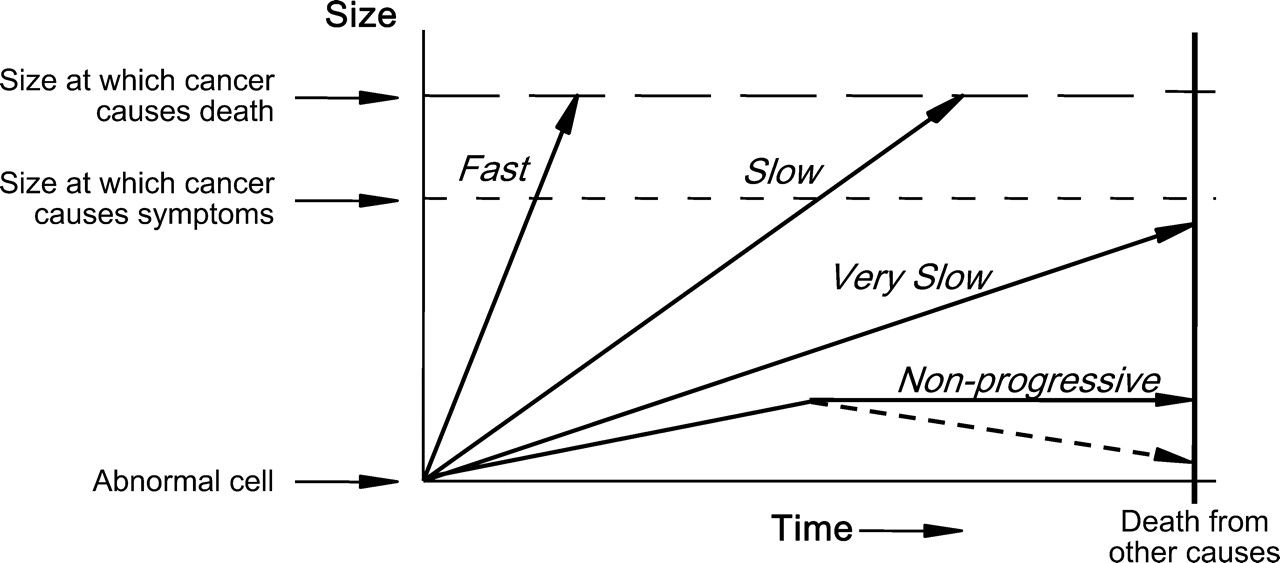
\includegraphics[width=\linewidth]{figures/heterogeneitypca.jpg}
\end{center}
\caption[Heterogeneity of prostate cancer progression]{Heterogeneity of prostate cancer progression. The arrow labeled ``fast'' represents a fast-growing cancer, one that quickly leads to symptoms and to death. The arrow labeled ``slow'' represents a slow-growing cancer, one that leads to symptoms and death but only after many years. The arrow labeled ``very slow'' represents a cancer that never causes problems because the patient will die of some other cause before the cancer is large enough to produce symptoms. The arrow labeled ``non-progressive'' represents cellular abnormalities that meet the pathological definition of cancer but never grow to cause symptoms. Reproduced with permission from \citet{welch_overdiagnosis_2010}.}
\label{fig:heterogeneitypca}
\end{figure}

\begin{figure}
\begin{center}
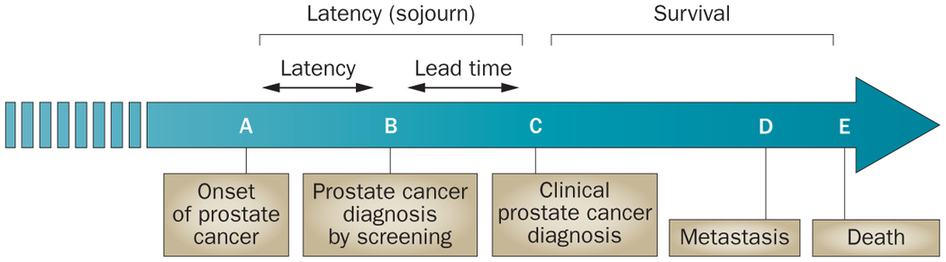
\includegraphics[width=\linewidth]{figures/naturalcourse.jpg}
\end{center}
\caption[Natural history of prostate cancer]{Natural history of prostate cancer. This figure illustrates the course of prostate cancer from initiation (A), to diagnosis by screening (B), to diagnosis by clinical symptoms (C), to clinically detectable metastatic disease (D), and finally to death from prostate cancer (E). Reproduced with permission from \citet{salinas_prostate_2014}.}
\label{fig:naturalcourse}
\end{figure}

% Descriptive epidemiology
\subsection{Descriptive epidemiology}
\label{section:descriptiveepidemiology}
\subsubsection{Incidence}
Prostate cancer was the second most common cancer in men worldwide and the most common one in more developed regions in 2012 \citep{ferlay_cancer_2015}. The age-standardized Incidence Rates (IRs) showed large geographic variation, with the highest rates observed in Australia/New Zealand (111.6 cases per 100,000 men), Northern America (97.2 cases per 100,000), and Western Europe (94.9 cases per 100,000 men). In contrast, the lowest IRs were observed in Asia (9.4 cases per 100,000 men) (figure \ref{fig:worldincpca}). Geographical differences were present also within Europe, where, for example, the age-standardized IR in Sweden was estimated to be around 1.7-times times of that in Italy \citep{ferlay_cancer_2015}.

\begin{figure}
\begin{center}
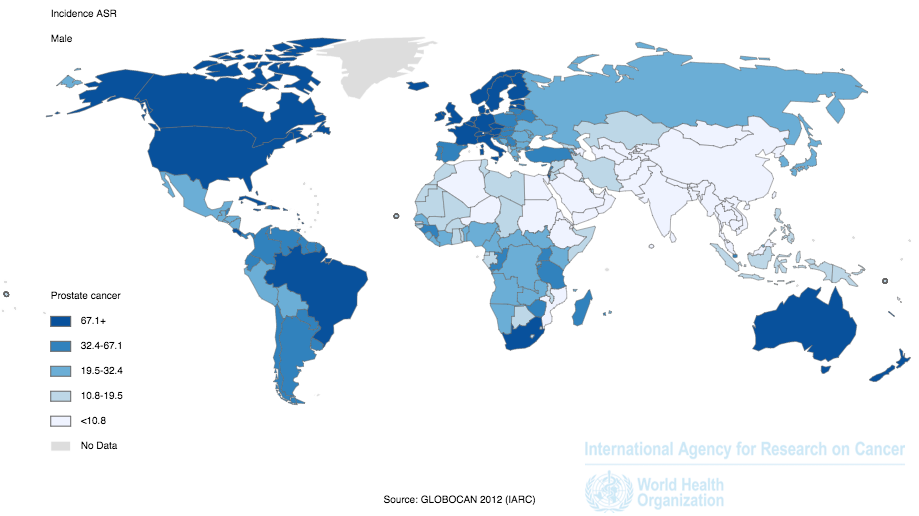
\includegraphics[width=\linewidth]{figures/incidencepca.png}
\end{center}
\caption[Age-standardized prostate cancer incidence rates per 100,000 men, worldwide, 2012]{Age-standardized prostate cancer incidence rates per 100,000 men, worldwide, 2012. Rates are age-standardized to the World population. Source: GLOBOCAN 2012 (IARC).}
\label{fig:worldincpca}
\end{figure}

In Sweden, the incidence of prostate cancer increased constantly during the period 1960--2004, with a steeper increase starting from the mid-1990's, and has been stable or even slightly decreasing since then (1.5\% average yearly decrease during 2004--2013) (figure \ref{fig:incmortsweden}). On average, around 10,000 cases were diagnosed every year during the period 2009--2013 and they amounted to 34\% of the total cancer diagnoses \citep{engholm_nordcan_2015}. Geographic variation is present also within Sweden, where an almost 2-fold difference in prostate cancer incidence was observed between counties according to NPCR data from 2000--2001 \citep{stattin_geographical_2005}.

\subsubsection{Mortality}
Prostate cancer was the fifth leading cause of cancer death in men worldwide in 2012, with an estimated total of 307,000 deaths (7\% of the overall male cancer mortality) \citep{ferlay_cancer_2015}. Geographical variation was less pronounced for mortality than for incidence (figure \ref{fig:worldmorpca}). Unlike incidence, the highest age-standardized Mortality Rates (MRs) were observed in populations of African descent. However, the lowest MRs were, similarly to incidence, observed in Asia (3.8 deaths per 100,000 men). Northern America showed slightly lower age-standardized MRs as compared with Europe (9.8 versus 11.3 deaths per 100,000 men) \citep{ferlay_cancer_2015}.

In Sweden, MRs have been relatively stable over time (figure \ref{fig:incmortsweden}), with a 2.7\% average yearly decrease during the period 2004--2013. Still, around 2,400 men died on average every year and accounted for 21\% of all cancer deaths (2009--2013) \citep{engholm_nordcan_2015}. The 5-year relative survival among men diagnosed with prostate cancer was around 90\%, while the 10-year survival was around 80\% (as of 2012), showing a steady increase over time \citep{socialstyrelsen_cancer_2013}. 

\begin{figure}
\begin{center}
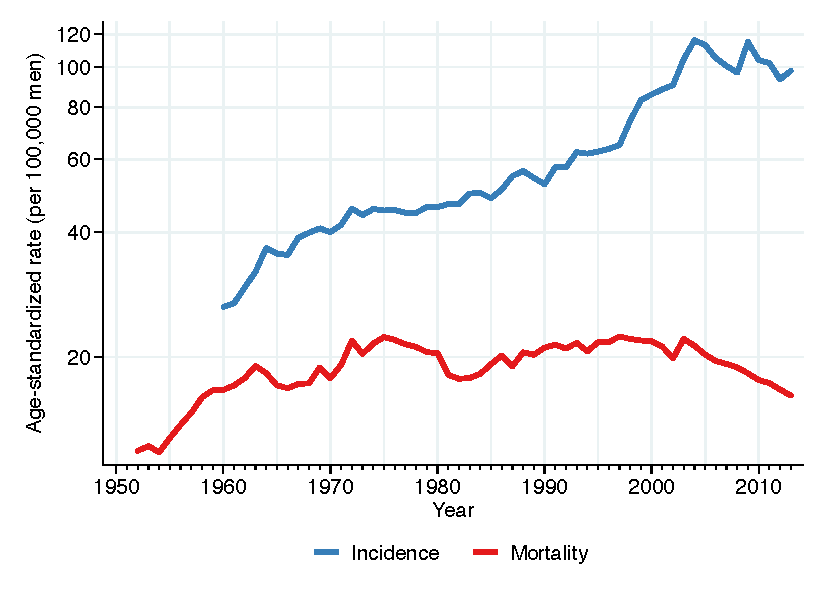
\includegraphics[width=\linewidth]{figures/incmortsweden.pdf}
\end{center}
\caption[Age-standardized prostate cancer incidence and mortality rates per 100,000 men, Sweden, 1952--2013]{Age-standardized prostate cancer incidence and mortality rates per 100,000 men, Sweden, 1952--2013. Rates are age-standardized to the World population. The vertical axis is on the natural log scale. Data source: NORDCAN.}
\label{fig:incmortsweden}
\end{figure}

\begin{figure}
\begin{center}
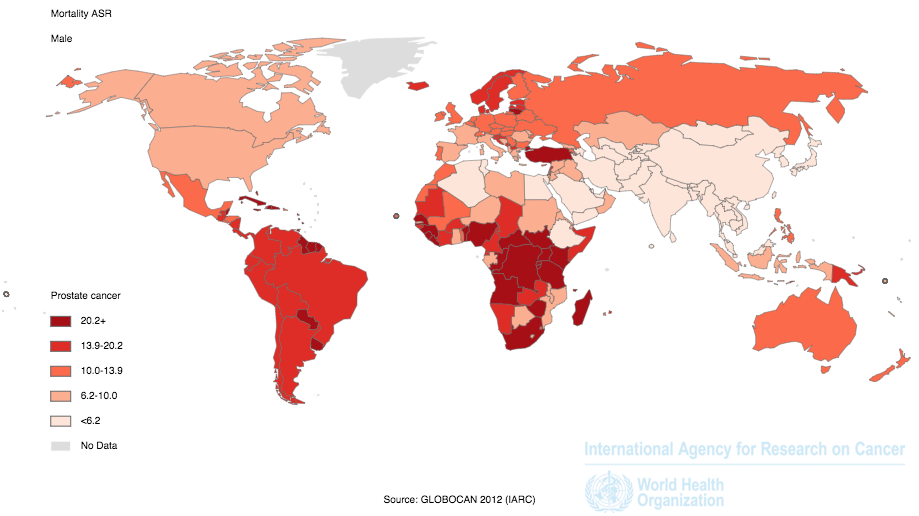
\includegraphics[width=\linewidth]{figures/mortalitypca.png}
\end{center}
\caption[Age-standardized prostate cancer mortality rates per 100,000 men, worldwide, 2012]{Age-standardized prostate cancer mortality rates per 100,000 men, worldwide, 2012. Rates are age-standardized to the World population. Source: GLOBOCAN 2012 (IARC).}
\label{fig:worldmorpca}
\end{figure}

% Classification of prostate cancer
\subsection{Classification}
\label{section:classification}
As a consequence of prostate cancer heterogeneity, its classification in risk categories at the time of diagnosis has the important objective of grouping patients with a similar prognosis. This allows primarily to make recommendations regarding their treatment, but also to compare clinical, pathological, and epidemiologic data coming from different sources. 

Different classification criteria have been developed with the aim of improving risk stratification \citep{cooperberg_university_2005, boorjian_mayo_2008, heidenreich_eau_2014, mohler_prostate_2014}. These criteria are generally based on a combination of Tumor Node Metastasis (TNM) staging system, Gleason grading system, and PSA serum level at diagnosis. In Sweden, the criterion used by the NPCR  is based on an adapted version of the National Comprehensive Cancer Network classification scheme and has been slightly modified during the last years \citep{npcr_prostatacancer_2013} (table \ref{table:classifpca}).

In practice, epidemiologic studies employ different and sometimes inconsistent criteria to classify prostate cancer. Moreover, the same terms are often used to refer to subtypes of cancer defined in different ways, thus complicating the interpretation and comparison of the results. For example, the term `advanced' prostate cancer is variably defined as higher grade, later stage, presence of metastatic disease or death, stage C or D on the Whitmore/Jewett scale, or different combinations of these.

\begin{table}[]
\centering
\caption[Risk categories according to the NPCR classification criteria]{Risk categories according to the NPCR classification criteria \citep{npcr_prostatacancer_2013}.}
\label{table:classifpca}
\begin{tabularx}{\textwidth}{rlX}
\hline
    &  {\bf Risk category}   &  \multicolumn{1}{c}{{\bf Criterion}}                                                                                                                    \\ \hline
1.  & Low-risk              & T1--2, Gleason Score 2--6, PSA \textless 10 \ngml                                                                               \\
1a. & Very low-risk         & T1c, PSA \textless 10 \ngml, Gleason Score 2--6, no more than 2 biopsy cores with cancer, total length of biopsies \textless 4mm \\
1b. & Low-risk (other)      & Low-risk not categorized as 1a                                                                                                    \\
1c. & Low-risk (missing)    & Missing information for low-risk categorization according to 1a and 1b                                                            \\
2.  & Intermediate-risk     & T1--2, Gleason Score 7, \textit{and}/\textit{or} 10 $\le$ PSA \textless 20 \ngml                                                                 \\
3a. & Localized high-risk   & T1--2, Gleason Score 8--10, \textit{and}/\textit{or} 20 $\le$ PSA \textless 50 \ngml                                                             \\
3b. & Locally advanced      & T3, PSA \textless 50 \ngml                                                                                                     \\
4.  & Regionally metastatic & T4 \textit{and}/\textit{or} N1 \textit{and}/\textit{or} 50 $\le$ PSA \textless 100 \ngml, \textit{and} Mx--0                                                                \\
5.  & Distant metastases    & M1 \textit{and}/\textit{or} PSA $\ge$ 100 \ngml                                                                                                  \\
6.  & Missing               & Missing information for categorization                                                                                            \\ \hline
\end{tabularx}
\end{table}

% PSA
\subsection{Prostate-specific antigen testing}
PSA is an enzyme produced by the prostate's epithelial cells and its primary function is to liquefy the semen in the seminal coagulum. Low PSA levels are present in the blood of healthy men and tend to increase naturally with age \citep{lilja_prostatespecific_2008}. However, abnormally high PSA levels may be a sign of prostate cancer or other prostatic diseases, such as benign prostatic hyperplasia or prostatitis --- that is, inflammation of the prostate. This reflects the fact that this enzyme is organ-specific but not prostate cancer--specific.

In the U.S., PSA testing was introduced in the late 1980s and approved by the Food and Drug Administration as a prostate cancer diagnostic marker in 1994 \citep{lilja_prostatespecific_2008}. The rationale behind this test is to detect prostate cancer early on, giving the possibility of intervening with curative treatments and, as a result, reduce the mortality from the disease. However, two problems related to the PSA test are its low sensitivity and the risk of overdiagnosis --- that is, the diagnosis of a cancer ``that would otherwise not go on to cause symptoms or death'' \citep{welch_overdiagnosis_2010}. Using data from the placebo arm of the Prostate Cancer Prevention Trial (PCPT), it was estimated that the test sensitivity is 24 and 35\% for cut-offs of 3 and 4 \ngml{}, respectively \citep{thompson_effect_2006}. More in general, PSA had a discrimination ability of 0.68, as measured by the area under the ROC curve \citep{thompson_effect_2006}. Overdiagnosis, which has been estimated to be in the range of 23--67\% for prostate cancer \citep{draisma_lead_2009, welch_overdiagnosis_2010}, can have a major impact on a man's life both in terms of psychological burden due to the cancer diagnosis and in terms of side effects following unnecessary treatment. Lastly, there is no conclusive evidence that PSA screening can in fact be useful to reduce prostate cancer mortality \citep{cuzick_prevention_2014}, and the two largest randomized trials on this matter --- the Prostate, Lung, Colorectal, and Ovarian Cancer (PLCO) screening trial, and the European Randomized Study of Screening for Prostate Cancer (ERSPC) trial ---  showed conflicting results. Namely, the PLCO trial observed no evidence of a decrease in prostate cancer mortality comparing systematic screening versus opportunistic screening, whereas the ERSPC trial observed a 21\% reduction in screened versus unscreened men. A recent study using data from Swedish registers showed that more-intense PSA screening decreased prostate cancer--specific mortality as compared with opportunistic screening, which might reconcile the findings from the PLCO  and ERSPC trials \citep{stattin_prostate_2014}. The value of using PSA as a screening tool in the general population remains however controversial \citep{cuzick_prevention_2014}.

Sweden does not have, to date, a national screening program for prostate cancer. Socialstyrelsen [the National Board for Health and Welfare (NBHW)] carried out an extensive literature review in 2013 and recommended against the introduction of a screening program \citep{socialstyrelsen_screening_2013}.\footnote{``Hälso- och sjukvården bör inte erbjuda screening för prostatacancer med test av prostataspecifikt antigen (PSA).''} Nevertheless, non-systematic, opportunistic PSA testing has increased over time since its introduction in the 1990s, which can explain the increase in prostate cancer incidence shown in figure \ref{fig:incmortsweden} \citep{jonsson_uptake_2011, nordstrom_prostatespecific_2013, socialstyrelsen_screening_2013}. It has been estimated that around half of the Swedish men aged 55--69 years old are PSA-tested, with large regional differences \citep{jonsson_uptake_2011}. In the Stockholm County, the proportion of the 2011 male population that had been tested during the previous 9 years was estimated to be between 46 and 77\%, depending on the age group considered \citep{nordstrom_prostatespecific_2013}.


% Risk factors
\subsection{Risk factors}
The etiology of prostate cancer is poorly understood, with the only established risk factors being age, family history of the disease, and race/ethnicity. To date, prostate cancer is not clearly linked to any preventable risk factors \citep{cogliano_preventable_2011,discacciati_lifestyle_2014, wcrf_continuous_2014}. 

At the same time, WCRF and AICR recently updated the findings from the 2007 Second Expert Report in their 2014 Continuous Update Project. The conclusions from the 2014 report read ``there is strong evidence that being overweight or obese increases the risk of advanced prostate cancer (being overweight or obese is assessed by body mass index (BMI), waist circumference and waist-hip ratio)'' \citep{wcrf_continuous_2014}. The degree of evidence for body fatness being associated with advanced prostate cancer, however, still does not reach the highest possible level of `strong evidence --- convincing'.

\subsubsection{Non-modifiable risk factors}
Age is the strongest risk factor for prostate cancer. Diagnosis is very uncommon in men younger than 40 years old and mortality is rare before the age of 50 years. It has been estimated that only 25\% of the incident cases in Europe in 2012 were diagnosed before the age of 65 years \citep{ferlay_cancer_2015}. Similarly, in Sweden, only 30\% of those men who received a prostate cancer diagnosis in 2013 were younger than 65 years of age \citep{socialstyrelsen_cancerincidens_2014}. Incidence of prostate cancer increases sharply after the age of 55 years, peaks around 70--74 years of age, and declines slightly thereafter \citep{ferlay_cancer_2015}. This steep trend in the age-incidence curve has been observed in multiple populations, including populations where PSA screening was completely absent \citep{armitage_age_1954}. Early-onset prostate cancer --- that is, prostate cancer diagnosed in men aged less than 55 years of age --- has been suggested to be a distinct phenotype, both from an etiological and clinical point of view \citep{salinas_prostate_2014}.

The risk of developing prostate cancer among men who have a first-degree relative with prostate cancer is around 2.5 times the risk among men without a diagnosed first-degree relative \citep{zeegers_empiric_2003, kicinski_epidemiological_2011}. This risk increases with decreasing age of the proband, with increasing number of affected relatives, and if the affected relative is a brother rather than the father. Family history is also associated to prostate cancer mortality \citep{brandt_agespecific_2010}. Familial aggregation of prostate cancer is largely due to genetic factors, as suggested by twin studies, where heritability was estimated to be around 30--40\%  \citep{ahlbom_cancer_1997, lichtenstein_environmental_2000, eeles_identification_2013}. In the last 10 years, more than 70 low-penetrance susceptibility loci have been identified through genome-wide association studies \citep{goh_germline_2014}. Familial aggregation can, however, be partly explained also by increased screening propensity among men with family history of prostate cancer \citep{bratt_effects_2010}.

Racial/ethnic variation in prostate cancer risk is very pronounced, too. In the U.S., during the period 2007--2011 (most recent available data), African-American men were observed to have around 60\% higher incidence and 140\% higher mortality as compared with Caucasian men. Conversely, Hispanic men had approximately 10\% lower incidence and  mortality \citep{acs_cancer_2015}. These differences are partially due to a combination of genetic and lifestyle factors, but disparities in socioeconomic status, as well as access to health care and prostate cancer screening may also contribute to explain the observed variation \citep{jones_explaining_2008}. Geographical variation is also substantial (figure \ref{fig:worldincpca}). Although this geographic variability can be explained by differences in screening programs and in genetic factors, results from migrant studies support the hypothesis that lifestyle factors might play a role in prostate cancer etiology \citep{wilson_lifestyle_2012}.

%TODO: add subsubsection on other modifiable risk factors?

\subsubsection{Body mass index}

Since body adiposity is related to both hormonal and metabolic pathways and since prostate cancer is a hormone-related cancer \citep{hsing_obesity_2007}, the investigation of a possible association between body fatness and prostate cancer risk has received considerable attention in epidemiologic research. The picture regarding this potential association has become clearer and more nuanced during the last 10 years or so.

BMI is probably the most common proxy for body adiposity in epidemiologic studies.\footnote{BMI is calculated as \kgmsq{} --- that is, weight in kilograms multiplied by height in meters to the power of minus 2.} In fact, weight and height can be measured relatively simply and accurately even in large populations unlike waist circumference or waist-to-hip ratio. BMI may be inadequate to measure body adiposity for a single individual, but it has been observed to correspond reasonably well with percentage body fat within sex and age groups \citep{flegal_comparisons_2009}.
 
By the late 2011,\footnote{The beginning of my graduate studies.} the existing body of literature on BMI and total prostate cancer was quite extensive, but at the same time results were inconsistent. In particular, the largest meta-analysis available to that date, which included 27 prospective studies for a total of more than 70 thousand prostate cancer cases, observed no evidence of an association between BMI and total prostate cancer [Relative Risk (RR) for every 5-unit increment: 1.03 (95\% Confidence Interval (CI): 0.99--1.06)]\footnote{The term `relative risk' will be used in this thesis as a generic term for the risk ratio, hazard rate ratio, incidence rate ratio, or odds ratio.} and a high between-study heterogeneity \citep{renehan_bodymass_2008}. Similarly, the 2007 Second Expert Report published by WCRF and AICR observed no evidence of an association, based on 24 prospective studies [RR for every 5-unit increment: 1.00 (95\% CI: 0.99--1.01)]. As a consequence, body fatness was listed among those factors for which no conclusions could be reached (strength of the evidence: `limited --- no conclusion') \citep[section~7.14]{wcrf_food_2007}. 

The hypothesis that the association between body adiposity and prostate cancer risk could differ according to the aggressiveness of the disease --- therefore suggesting etiological heterogeneity of prostate cancer related to obesity --- repeatedly appeared in the literature during those years  \citep{freedland_are_2006, freedland_obesity_2007, hsing_obesity_2007, hsing_androgen_2008}. The available epidemiologic evidence supported this intriguing hypothesis, but at the same time it was still limited. In fact, just a few studies had looked into the association between body adiposity and prostate cancer by subtype of the disease. As a result, the only available meta-analysis  that carried out separate analyses by subtype of prostate cancer included 4 case-control and 6 prospective studies (two of which were very small), for a total of less than 2 thousand cases. Despite this, a positive association between BMI and the risk of advanced prostate cancer was observed [RR for every 5-unit increment: 1.12 (95\% CI: 1.01--1.23)] \citep{macinnis_body_2006}.

During the years following the meta-analysis by \citet{macinnis_body_2006} and the Second Expert Report \citep{wcrf_food_2007}, a considerable amount of epidemiologic research on body adiposity and prostate cancer has been carried out, including \citetalias{discacciati_body_2011} of this thesis. Furthermore, epidemiologic studies started to systematically report results separately by specific subtypes of prostate cancer, although with the limitations described in section \ref{section:classification}, allowing a clearer picture to emerge. \citetalias{discacciati_body_2012} was the first meta-analysis after the one published by \citet{macinnis_body_2006} to summarize the available evidence on BMI and prostate cancer risk by subtype of the disease. In particular, \citetalias{discacciati_body_2012} was considerably larger, including 13 prospective studies and about 6 times the number of prostate cancer cases. Results showed an increased risk of advanced prostate cancer [RR for every 5-unit increment: 1.09 (95\% CI: 1.02--1.16)] and a decreased risk of localized prostate cancer [RR for every 5-unit increment: 0.94 (95\% CI: 0.91--0.97)]. Lastly, the 2014 Continuous Update Project report showed very similar results to those of \citetalias{discacciati_body_2012} for advanced prostate cancer [RR for every 5-unit increment: 1.08 (95\% CI: 1.04--1.12)], while a non-linear association was observed for localized prostate cancer \citep{wcrf_continuous_2014}. An overview of the results from meta-analyses on BMI and prostate cancer incidence --- including the updated dose--response meta-analysis based on \citetalias{discacciati_body_2012} and described in section \ref{section:results4updated} --- is reported in table \ref{table:summarybmi}.


\begin{sidewaystable}[]  
\centering
\begin{threeparttable}
\caption[Meta-analyses on BMI and incidence of prostate cancer]{Results from dose--response meta-analyses on BMI and incidence of prostate cancer.}
\label{table:summarybmi}
\begin{tabular}{lllccc}
\hline
{\bf Outcome} & \multicolumn{1}{c}{{\bf Year}} & {\bf Authors} & \multicolumn{1}{c}{{\bf Number of studies}} & {\bf RR}\tnote{a,b} & {\bf 95\%  CI} \\ \hline
Total prostate cancer  & \citeyear{wcrf_food_2007} & \citeauthor{wcrf_food_2007} & 24 cohort & 1.00 & 0.99--1.01 \\
 & \citeyear{renehan_bodymass_2008} & \citeauthor{renehan_bodymass_2008} & 27 cohort & 1.03 & 0.99--1.06 \\
 & \citeyear{wcrf_continuous_2014} & \citeauthor{wcrf_continuous_2014} & 39 cohort & 1.00 & 0.97--1.03 \\
 &  &  &  & \multicolumn{1}{l}{} & \multicolumn{1}{l}{} \\
Localized prostate cancer & \citeyear{macinnis_body_2006} & \citeauthor{macinnis_body_2006} & 6 cohort and 4 case-control & 0.96 & 0.89--1.03 \\
 & \citeyear{discacciati_body_2012} & \citeauthor{discacciati_body_2012} \citepalias{discacciati_body_2012} & 12 cohort & 0.94 & 0.91--0.97 \\
 & \citeyear{wcrf_continuous_2014} & \citeauthor{wcrf_continuous_2014} & 14 cohort & ---\tnote{c,d} & --- \\
 & 2015 & Discacciati \citepalias[updated]{discacciati_body_2012} & 14 cohort & ---\tnote{c,e} & --- \\
 &  &  &  & \multicolumn{1}{l}{} & \multicolumn{1}{l}{} \\
Advanced prostate cancer & \citeyear{macinnis_body_2006} & \citeauthor{macinnis_body_2006} & 6 cohort and 4 case-control & 1.12 & 1.01--1.23 \\
 & \citeyear{discacciati_body_2012} & \citeauthor{discacciati_body_2012} \citepalias{discacciati_body_2012} & 13 cohort & 1.09 & 1.02--1.16 \\
 & \citeyear{wcrf_continuous_2014} & \citeauthor{wcrf_continuous_2014} & 23 cohort & 1.08 & 1.04--1.12 \\ 
  & 2015 & Discacciati \citepalias[updated]{discacciati_body_2012} & 18 cohort & 1.07 & 1.03--1.12 \\ \hline
\end{tabular}
\begin{tablenotes}
\item [a] \footnotesize For every 5-unit increment in BMI.
\item [b] \footnotesize Results are from random-effect meta-analyses.
\item [c] \footnotesize No RR for every 5-unit increment in BMI was calculated, as there was evidence of a non-linear relationship.
\item [d] \footnotesize The RRs for 25, 31, and 37 \kgmsq{} versus 21 \kgmsq{} were 1.04 (95\% CI: 1.02--1.05), 0.94 (95\% CI: 0.92--0.96), and 0.79 (95\% CI: 0.75--0.83), respectively ($p_{\textrm{non-linearity}}<0.01$). 
\item [e] \footnotesize The RRs for 25, 30, and 35 \kgmsq{} versus 22 \kgmsq{} were 1.01 (95\% CI: 0.99--1.04), 0.93 (95\% CI: 0.90--0.98), and 0.81 (95\% CI: 0.74--0.88), respectively ($p_{\textrm{non-linearity}}<0.001$). 
\end{tablenotes}
\end{threeparttable}
\end{sidewaystable}

In conclusion, the official recommendations issued in 2014 by the WCRF and ARIC read ``to reduce the risk of developing advanced prostate cancer, we recommend maintaining a healthy weight'' \citep{wcrf_continuous_2014}.

Given that prostate cancer has usually a long latency period, spanning even decades between tumor initiation and diagnosis, body adiposity earlier in life could in theory play an important role in tumor initiation and development. Moreover, the prostate may be more susceptible to carcinogenic exposures during the developmental stages and immediately thereafter \citep{sutcliffe_prostate_2013}. For these reasons, BMI during childhood, puberty, and early adulthood --- defined as ages between 18 and 30 years  --- has been investigated by epidemiologic studies, including \citetalias{discacciati_body_2011} of this thesis. The results, however, are inconsistent  \citep{sutcliffe_prostate_2013}. 
\newpage %TODO: hard coding
